\subsection{Постановка задачи}
3.3. Для таблично заданной функции путем решения нормальной системы МНК найти приближающие многочлены a) 1-ой  и б) 2-ой степени. Для каждого из приближающих многочленов вычислить сумму квадратов ошибок. Построить графики приближаемой функции и приближающих многочленов.

{\bfseries Вариант:} 19
    \begin{center}
        \begin{tabular}{ |c|c|c|c|c|c|c| } 
			 \hline
			 $i$ & 0 & 1 & 2 & 3 & 4 & 5 \\ 
			 \hline
			 $x_i$ & -0.7 & -0.4 & -0.1 & 0.2 & 0.5 & 0.8 \\ 
			 \hline
			 $y_i$ & -1.4754 & -0.81152 & -0.20017 & 0.40136 & 1.0236 & 1.7273 \\ 
			 \hline
        \end{tabular}
    \end{center}
\pagebreak

\subsection{Результаты работы}
\begin{figure}[h!]
\centering
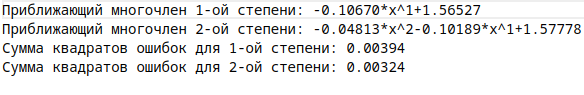
\includegraphics[width=.5\textwidth]{lab3.3}
\caption{Вывод в консоли}
\end{figure}


\subsection{Исходный код}
\lstinputlisting[title=\texttt{Lab3.3.cpp}]{../stud/saifullin/task3.3/Lab3.3.cpp}
\pagebreak

